\chapter{Il Cloud e le sue sfaccettature}

\section{Cloud Computing}
La differenza tra il possedere e l'utilizzare. E' questo l'aspetto cruciale del cambiamento apportato dal cloud computing rispetto al software tradizionale. Le risorse, che siano quelle di archiviazione, elaborazione o altro, non sono mai ad hoc per un singolo utilizzatore, ma vengono assegnate on demand e appartengono ad un insieme condiviso da tutti gli altri utenti del prodotto. Attraverso internet ogni utente può accedere a queste risorse in qualsiasi momento. Tali risorse vengono opportunamente allocate in maniera dinamica e completamente automatizzata. Si possono utilizzare così anche software non installati sul proprio computer o usufruire di una memoria di massa accessibile da qualsiasi dispositivo.
\paragraph{}
L'esperienza utente che si vuole fornire però è quella di un utilizzo esclusivo della risorsa, come nei software tradizionali. In realtà la risorsa viene solo sapientemente distribuita tra tutti coloro che la richiedono. Ciò fa si che, potenzialmente, un singolo utente possa acquisire risorse notevolmente maggiori rispetto ai software che utilizzano la macchina locale.
\begin{figure}
	\centering
	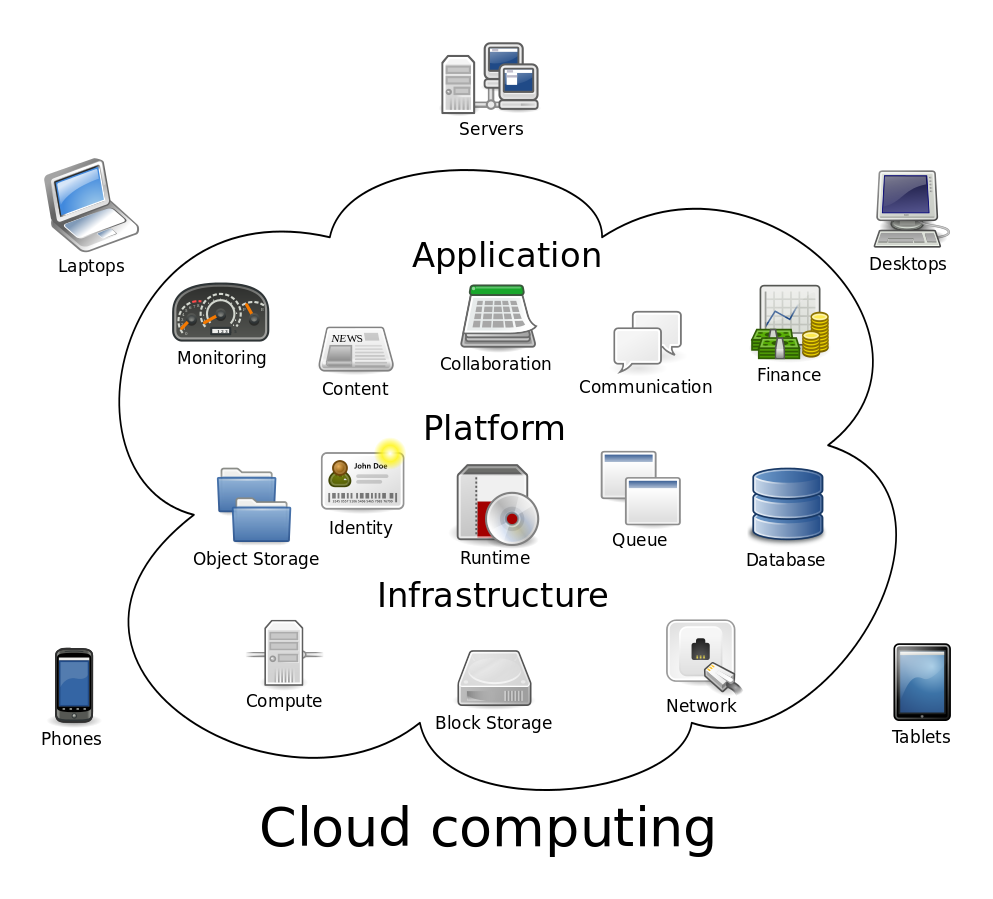
\includegraphics[width=0.5\linewidth]{capitoli/imgs/CloudComputing}
	\caption{Diagramma logico di una rete Cloud Computing}
	\label{fig:cloudcomputing}
\end{figure}
\subsection{Vantaggi del Cloud Computing}
\begin{itemize}
	\item Costo: \\
	Con l'avvento del cloud tutta la gestione dell'infrastruttura sottostante al software diviene a carico del provider. Vengono eliminate spese per la gestione dei data center locali. Facendo riferimento alla versione SaaS di BigFix ad esempio, il cliente viene sollevato dal pesante onere di utilizzare server locali e gestirne le relative connessioni. Il provider ospita tutto l'hardware di cui il cliente ha bisogno.
	
	\item Facilità di installazione: \\
	Anche qui ci risulta molto utile prendere come esempio la suite di BigFix. Quando un nuovo cliente acquista il prodotto nella sua versione on-premises, un'incaricato di IBM si reca presso il cliente e lì inizia un processo di installazione della suite che può impiegare diverse ore. Nello scenario SaaS il cambiamento è radicale. E' sufficiente che il cliente compili una form online, dopo alcuni minuti poi riceve una mail con il link per accedere al servizio.
	
	\item Prestazioni \\
	Una delle motivazioni principali per la quale si sceglie di fare uso del clud computing sono proprio le prestazioni, soprattutto se si adotta il paradigma PaaS. Richiedendo tramite cloud le risorse di calcolo, si può fare affidamento a dei provider che fanno dei server ad alte prestazioni il loro punto di forza. L'utente può, in questo modo, abbattere dei bottleneck che altrimenti risulterebbero di grande impedimento. Nel 2016 IBM mette per la prima volta a disposizione pubblicamente un computer quantistico, proprio attraverso una piattaforma cloud (IBM Q). Questo può rappresentare un esempio estremo in ottica prestazioni, ma che può rendere un'idea di quale potrà essere il trend nei prossimi anni.
	
	\item Affidabilità \\
	Operazioni di mirroring da parte dei provider dei servizi cloud fa sì che il backup dei dati sia continuo ed economico. Molto spesso i provider hanno data center sparsi in molte parti del mondo, ciò aumenta la resistenza a guasti o addirittura catastrofi che possono verificarsi. Ovviamente questo grado di replicazione dei servizi è impensabile nella fruizione on premise dei prodotti.
\end{itemize}

\section{Tipologie di servizi Cloud}
Il termine Cloud risulta essere in realtà molto generico. Esso comprende diverse tipologie di fornitura dei servizi, a seconda della risorsa che viene offerta dal provider. La maggior parte dei servizi di Cloud Computing rientrano in tre tipologie principali: Infrastruttura distribuita come Servizio (IaaS, Infrastructure as a Service), Piattaforma distribuita come Servizio (PaaS, Platform as a Service) e Software come un Servizio (SaaS, Software as a Service). Oltre a queste tipologie, annoveriamo anche altre soluzioni come il DaaS (Data a a Service) e l'HaaS (Hardware as a Service). Andiamo a vedere nel dettaglio come, a seconda della modalità di utilizzo del paradigma Cloud, queste strategie si differenziano. 
\begin{figure}
	\centering
	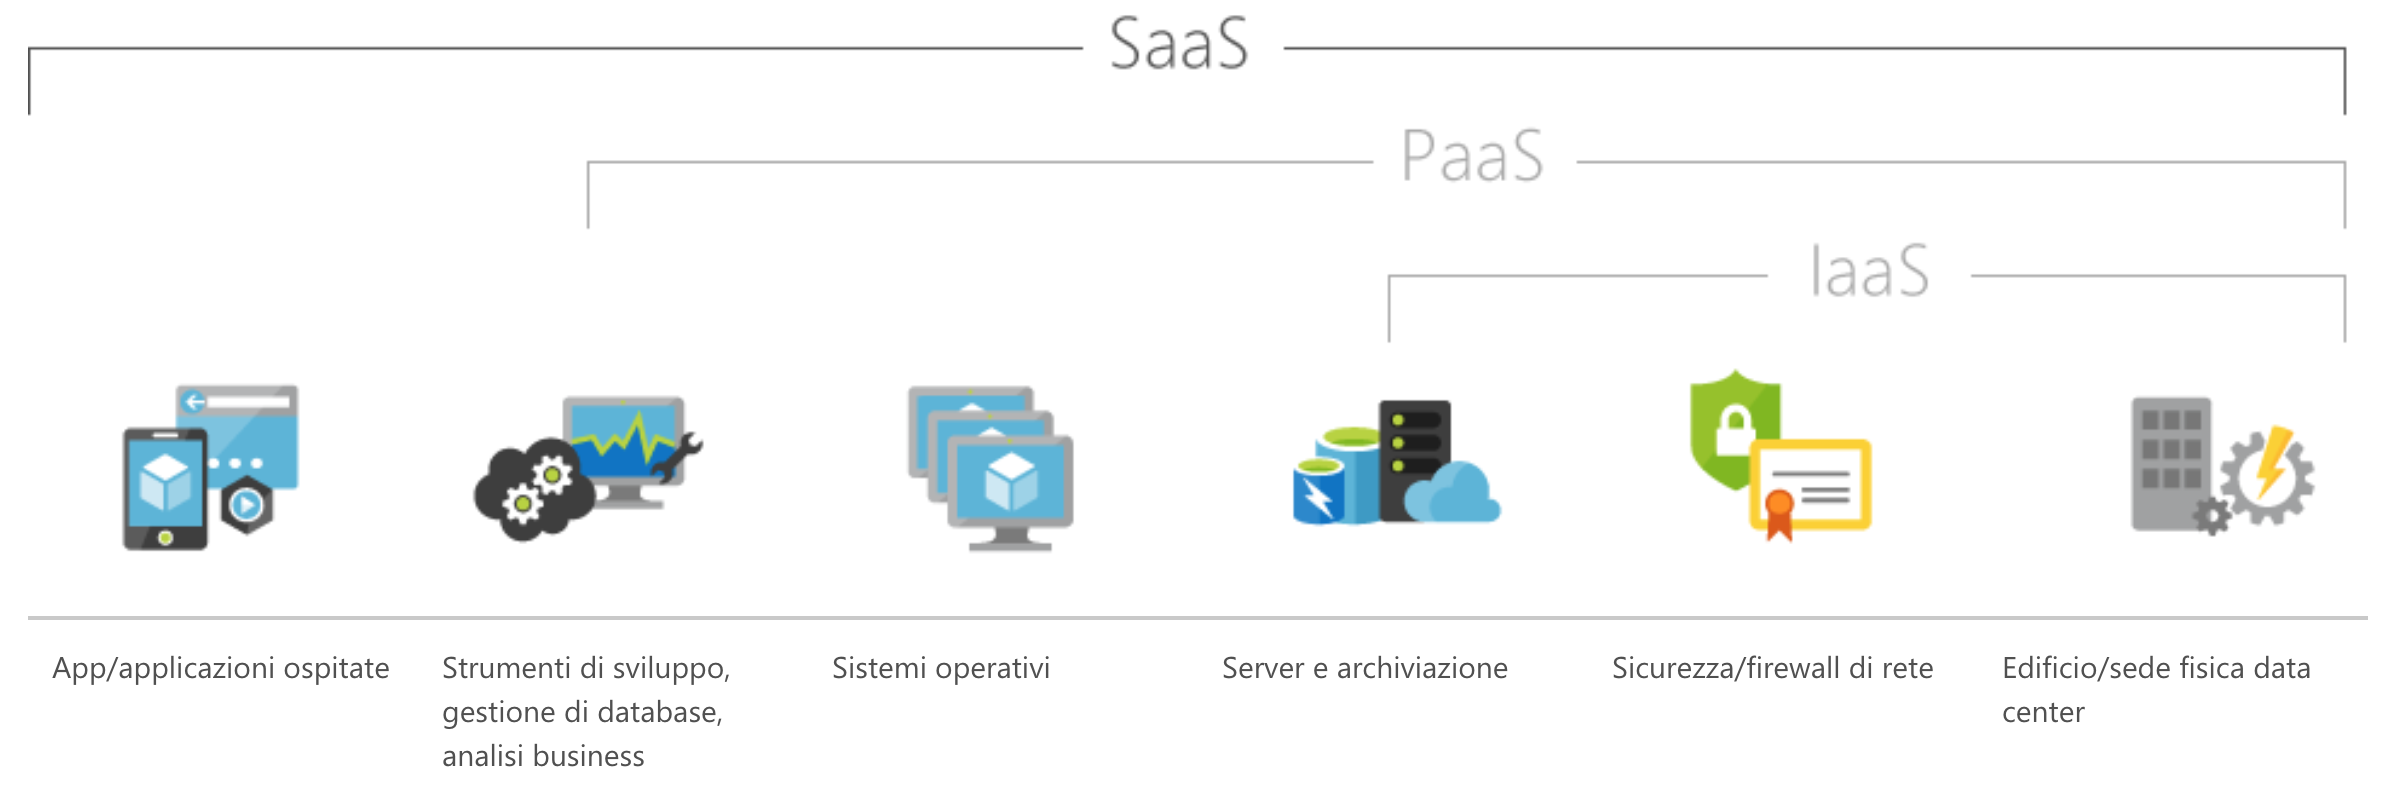
\includegraphics[width=0.7\linewidth]{capitoli/imgs/TipologieCloud}
	\caption{Panoramica delle principali tipologie Cloud}
	\label{fig:tipologiecloud}
\end{figure}

\subsection{IaaS, Infrastructure as a Service}
E' la tipologia più basilare. Vengono messe a disposizione piattaforme di elaborazione. Utilizzando un IaaS si affittano le infrastrutture utili ai propri scopi, come ad esempio server, macchine virtuali (VMs), risorse di archiviazione, reti e sistemi operativi. Può, inoltre, essere messo a disposizione anche hardware in remoto. Il provider di servizi cloud gestisce l'infrastruttura, mentre l'utente acquista, installa, configura e gestisce il software, tra cui sistemi operativi, middleware e applicazioni.
\paragraph{Vantaggi}
Una soluzione IaaS è quella che garantisce maggiore flessibilità. Tra i vantaggi principali ricordiamo:
\begin{itemize}
	\item  Elevata scalabilità \\
	Il modello IaaS permette una scalabilità verticale rapida ed economica
	\item Rapidità di innovazione \\
	Nel caso del lancio di un nuovo prodotto basato sulla piattaforma IaaS, il tempo di attesa per le nuove configurazioni infrastrutturali è solamente dell'ordine di pochi minuti.
	\item Adattabilità alle richieste \\
	Un modello IaaS è estremamente flessibile alle variazioni delle richieste. Si possono facilmente aumentare le risorse nei momenti di picco e ridurle quando non è necessario, risparmiando quindi denaro.
	
\end{itemize}
\subsection{PaaS, Platform as a Service}
Una piattaforma distribuita come servizio (PaaS, Platform as a Service) è un ambiente cloud di sviluppo completo. Una soluzione PaaS è progettata per consentire il ciclo completo dello sviluppo delle applicazioni: creazione, test, distribuzione, gestione e aggiornamento. L'utente ha tutta la libertà di sviluppare gli applicativi a proprio piacimento, ma lavora con componenti software già pronti all'utilizzo (i microservices). Questi componenti non sono localizzati presso chi utilizza il cloud, bensì presso il provider, il quale si occupa del loro mantenimento e aggiornamento. Il modello PaaS consente di evitare le spese e la complessità legate all'acquisto e alla gestione di licenze software, middleware e infrastruttura delle applicazioni sottostanti o strumenti di sviluppo. L'utente gestisce le applicazioni e i servizi che sviluppa e il provider cloud si occupa di tutto il resto.
\paragraph{Vantaggi}
Uno scenario PaaS riduce quindi notevolmente la quantità di codice da scrivere semplificando quindi il lavoro dello sviluppatore e aumentandone la produttività. Inoltre risulta molto più semplice così il porting di un prodotto da web a mobile e viceversa. Componenti molto complessi e costosi possono essere messi a disposizione, con un utilizzo limitato, anche per sviluppatori che altrimenti non potrebbero permetterselo. 
\subsubsection{IBM Bluemix}
Troviamo, sempre all'interno di IBM, uno dei principali servizi cloud PaaS presenti sul mercato: IBM BlueMix. L'utente può usufruire di un'astrazione di molte componenti utili allo sviluppo. Si può, ad esempio, fare uso di Database specifici, di moduli dedicati all'IoT, di tecnologie Blockchain e molto altro. Ne vediamo alcuni esempi nella figura 3.3
\begin{figure}[h!]
	\centering
	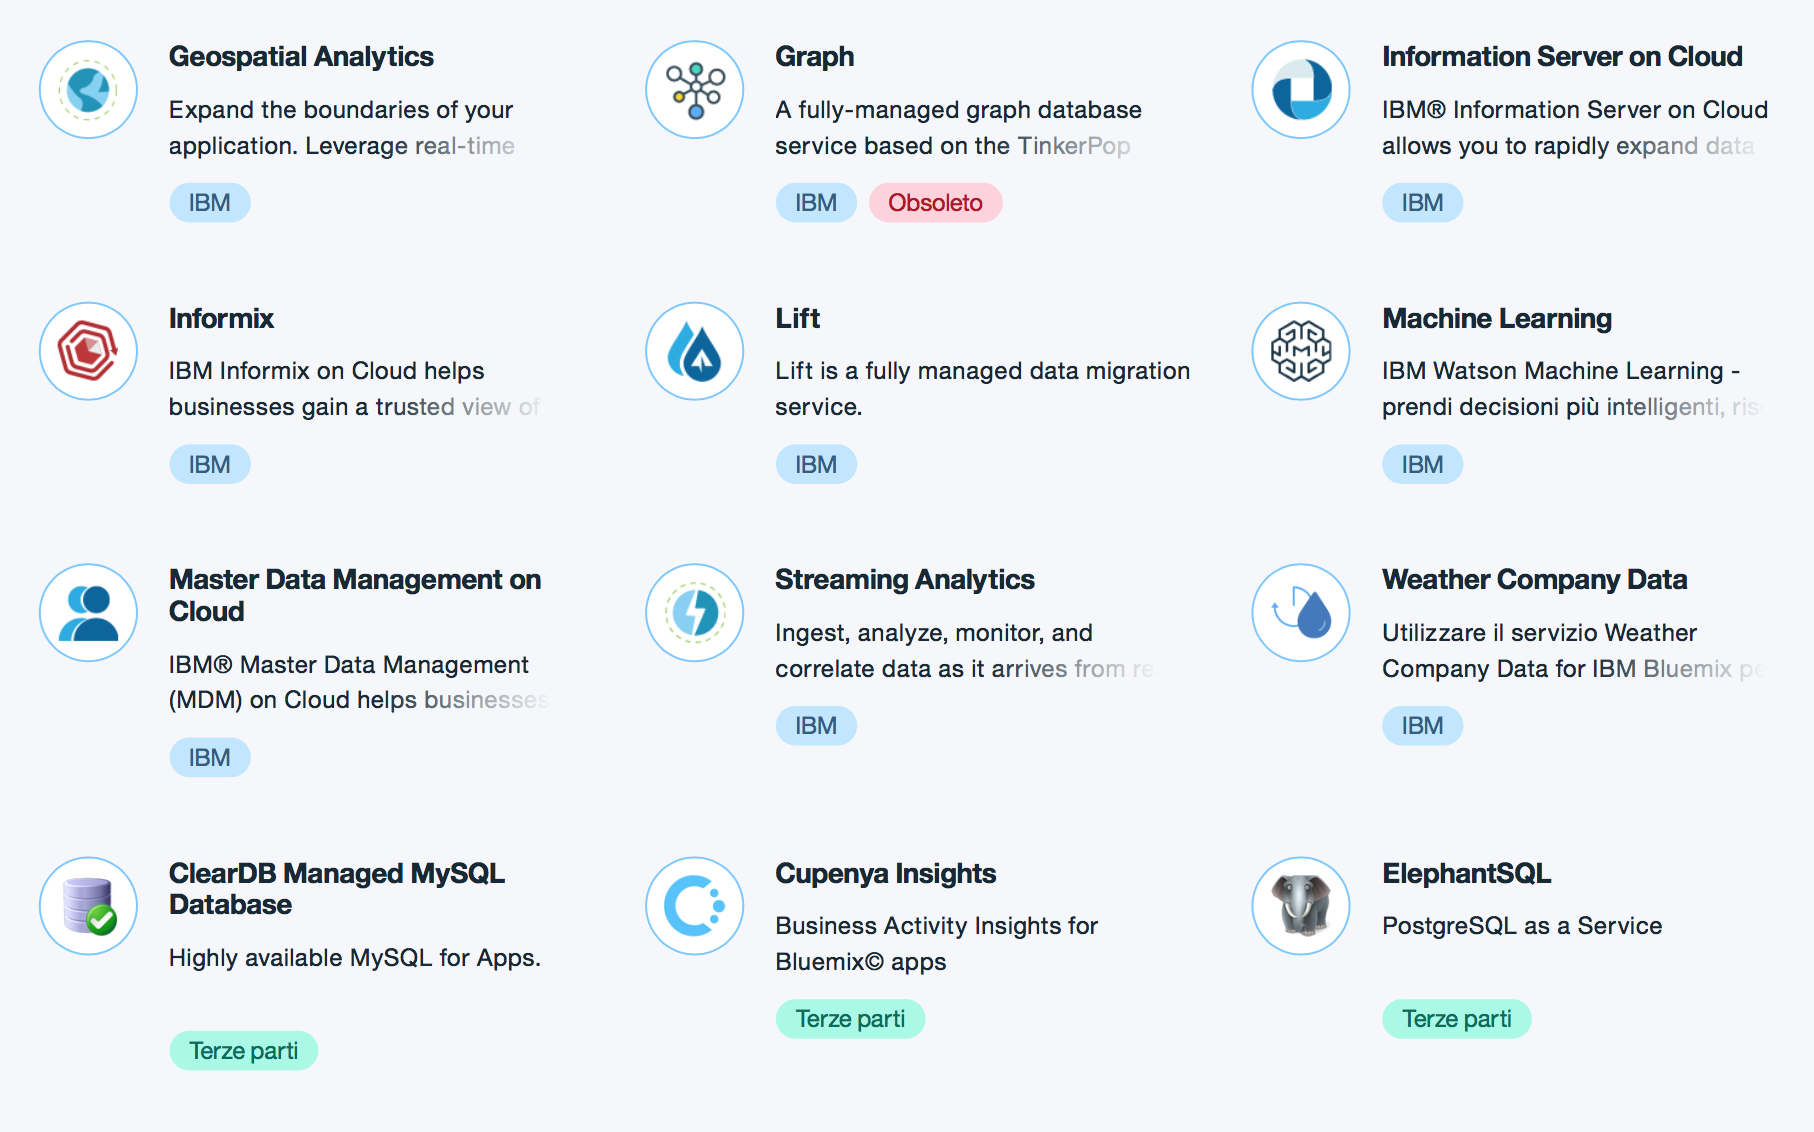
\includegraphics[width=\textwidth,keepaspectratio=true]{capitoli/imgs/catalog.png}
	\caption{Esempi di moduli presenti nel catalogo BlueMix}
\end{figure}
\subsubsection{IBM Watson}
Tra le componenti sviluppate da IBM merita una menzione anche Watson. Watson è un sistema di intelligenza artificiale in grado di rispondere a domande espresse in un linguaggio naturale. Tra le funzionalità ci sono quelle di elaborazione del linguaggio naturale, information retrieval, rappresentazione della conoscenza, ragionamento automatico e tecnologie di apprendimento automatico.
\begin{figure}[h!]
	\centering
	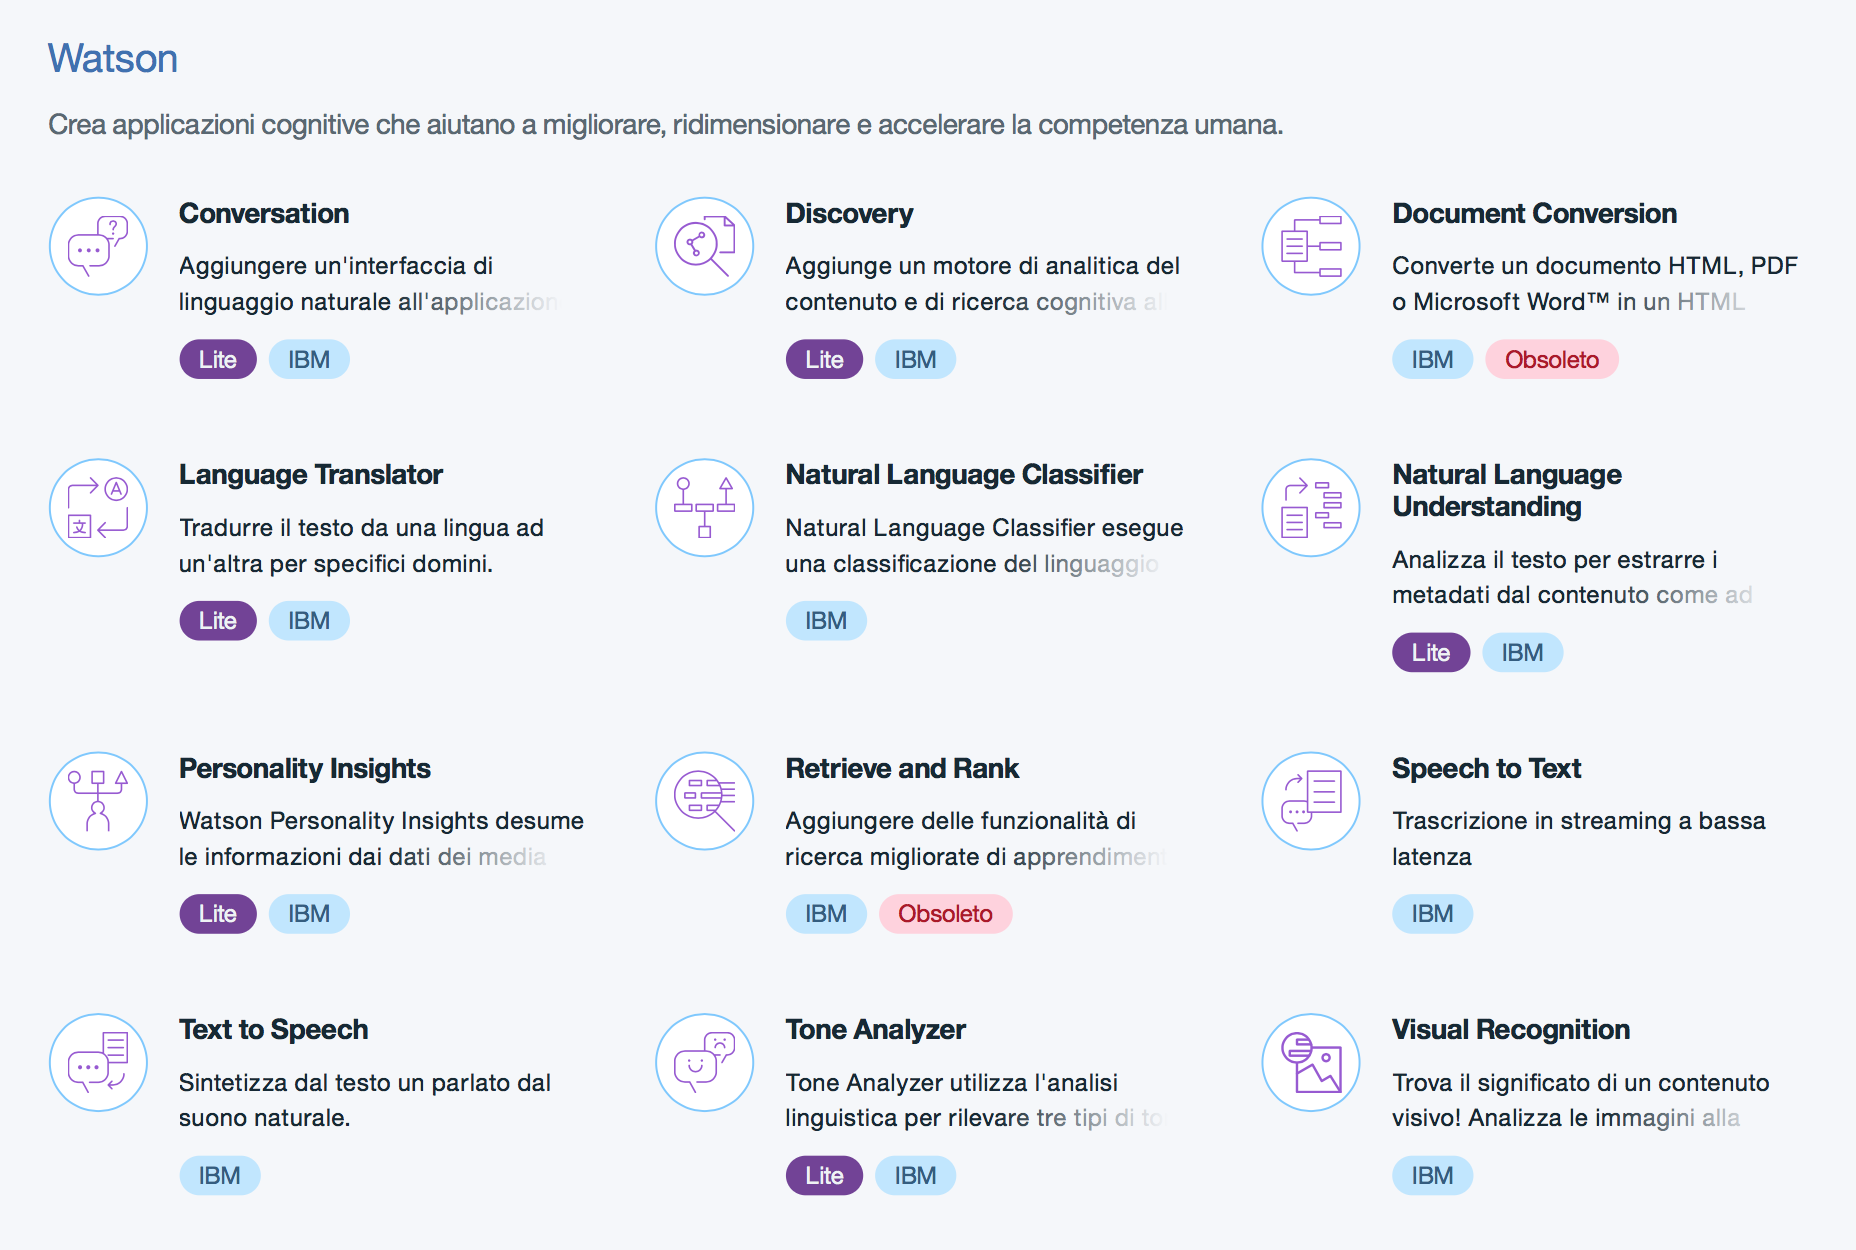
\includegraphics[width=\textwidth,keepaspectratio=true]{capitoli/imgs/watson.png}
	\caption{Alcuni moduli Bluemix appartenenti a Watson}
\end{figure}

\subsection{SaaS, Software as a Service}

Il Software as a Service (SaaS) è un modello di distribuzione del software in cui l'applicativo e gli eventuali servizi collegati sono eseguiti in un ambiente centralizzato e gli utenti vi accedono via rete, quasi sempre via Internet e usando un browser come interfaccia. I SaaS sono ormai sempre più diffusi. Tra i maggiori si ricordano le Google Apps (ad esempio Gmail, Google Drive, Google Calendar) e la suite Microsoft Office 365. Con la metodologia SaaS il provider fornisce tutto il software direttamente all'utente, al quale non resta che usarlo senza preoccuparsi di installazioni e configurazioni. L'utente non paga per il possesso del software, ma per il suo utilizzo. A volte vengono infatti applicate tariffe in base all'utilizzo del prodotto stesso. 

\paragraph{}
Spesso un'architettura SaaS è multi-tenant, ossia una sola applicazione server viene utilizzata da più utenti mantenendone, al tempo stesso, separati gli ambienti e i dati. Il concetto di multi-tenancy verrà approfondito maggiormente nei prossimi capitoli.
\paragraph{}
Attualmente le principali software house attive nel mondo aziendale traggono dalle offerte SaaS circa il venti percento del loro fatturato, nel giro di tre-quattro anni la maggior parte di loro prevede che il mercato SaaS diventi sempre più fondamentale.

\subsubsection{Vantaggi}
\paragraph{}
Con la metodologia SaaS il provider fornisce il software all'utente già pronto all'uso, l'utente non si deve quindi preoccupare di nient'altro. I clienti non pagano più per il possesso del software, ma per l'utilizzo dello stesso. In questo modo spesso possono essere notevolmente abbattute le spese iniziali per l'installazione e la configurazione di un prodotto, sostituendole con un costo di funzionamento. Il SaaS comporta quindi una spesa inferiore, ma ricorrente. E' il vendor però a preoccuparsi della manutenzione.
\paragraph{}
La caratteristica preponderante del cloud SaaS è proprio quella di poter raggiungere i propri dati personali da qualunque luogo e con qualunque dispositivo. E' questa la vera rivoluzione del cloud nel senso più comune del termine. Quando si ha bisogno di lavorare con i propri dati personali, non si ha più la necessità di avere con se hardware specifico, il proprio laptop o la propria usb key, ma basta avere le proprie credenziali al accedere così allo spazio dedicato. 
\paragraph{}
L'accesso alle tecnologie più sofisticate diviene inoltre alla portata di tutti. Software come gli ERP (Enterprise Resource Planning) e i CRM(Customer Relationship Management), possono essere utilizzati anche da quelle organizzazioni che prima non potevano permettersi un investimento di questo tipo.
\paragraph{} 
Un elemento che contraddistingue il SaaS è il notevole grado di apertura verso altre componenti, il che le rende altamente riusabili e flessibili, ciò è ovviamente un grande punto di forza in quanto i requisiti dell'utente spesso cambiano in continuazione.
\paragraph{}
Gli scenari di aggiornamento cambiano radicalmente. La distribuzione degli aggiornamenti è pressoché immediata e tutti gli utenti hanno la certezza di operare con l'ultima versione del software. Le fasi di upgrading non comportano più l'assenza del servizio come nella versione on premise. L'utente non si accorge neanche del processo di aggiornamento e si ritrova ad utilizzare il software aggiornato.
\subsubsection{Svantaggi}
\paragraph{}
Il modello ha ovviamente anche i suoi svantaggi, o perlomeno alcune criticità che vanno tenute presenti. La principale sta nella gestione dei dati aziendali, che sono localizzati nei data center del cloud provider e questo può essere giudicato un rischio per la privacy delle informazioni o addirittura costituire una violazione delle norme che devono osservare le aziende operanti in settori particolari come, ad esempio, la sanità e la difesa.
\paragraph{}
Tra gli altri aspetti di cui tenere conto ci sono sicuramente le prestazioni e l'affidabilità delle connessioni, che risultano essere i veri bottleneck non solo delle soluzioni SaaS, ma di tutte le soluzioni cloud. 
\paragraph{}
Infine altre criticità riguardano il provider dei servizi. Bisogna tenere conto quanto sia affidabile e se presenta, ad esempio, il rischio che esca dal mercato o ritiri il prodotto software SaaS. 

\begin{figure} [h!]
	\centering
	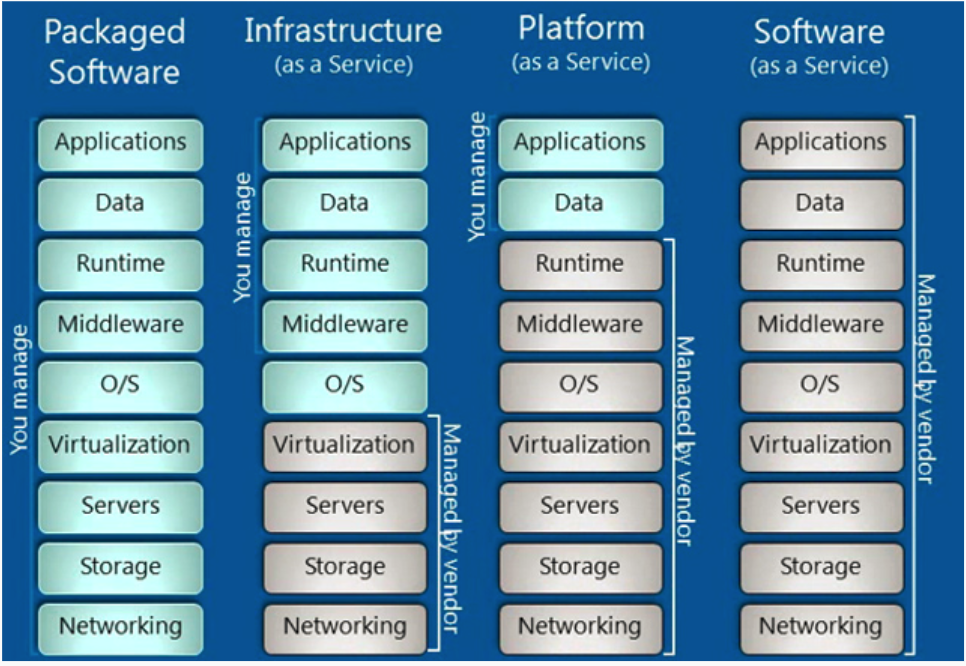
\includegraphics[width=0.7\linewidth]{capitoli/imgs/cloudstacks.png}
	\caption{Confronto di riepilogo tra i paradigmi cloud e il prodotto on premise}
\end{figure}


\section{SOA, Service Oriented Architecture}
Il concetto di Service Oriented Architecture è affine a quello di SaaS. Un SaaS può rappresentare la percezione da parte dell'utente della modalità di utilizzo di una Architettura Service Oriented. Un servizio ha l'obiettivo di incapsulare una ben precisa funzionalità, per renderla disponibile e accessibile come servizio software sul web. L'Architettura Orientata ai Servizi è quindi uno stile architetturale per la costruzione di una molteplicità di sistemi o applicazioni sulla base della composizione di un insieme di servizi. Spesso, quindi, queste applicazioni non fanno altro che comporre un SaaS, il quale trova in un'architettura di questo tipo una appropriata implementazione.
\section{Il software On Premise}
Abbiamo appena analizzato le peculiarità delle singole tipologie di servizi cloud. Anche il classico modello on premise però ha i suoi punti di forza.
\paragraph{Vantaggi del Software On Premise}
\begin{itemize}
	\item Controllo esclusivo su sistemi e dati
	\item Alta personalizzazione
	\item Gestione interna dei dati sensibili
	\item Alto investimento iniziale ammortizzato nel lungo periodo
\end{itemize}

\paragraph{}
Nel caso in cui si abbiano già a disposizione tutte le infrastrutture necessarie, non risulta più vero che la soluzione cloud sia la più economica per far fronte alla necessità di un determinato applicativo. E' anche necessario però che il software sia abbastanza centralizzato per adottare una soluzione on premise e questo può rappresentare un rischio per la fault tolerance.

\paragraph{}
Occorre quindi fare un'analisi di quanto sia necessario personalizzare il software di cui si ha bisogno e averne il pieno controllo come nella modalità onpremise, tenendo conto che un software on premise richiede molta più cura, manutenzione e lavoro di una soluzione basata su cloud. Il paradigma di fornitura on premise risulta ancora essere la soluzione più adatta nel caso in cui la gestione diretta dei dati sia fondamentale per policy aziendali oppure sia necessaria una maggiore flessibilità di configurazione per l'integrazione con altre architetture software. Un'altro requisito che ne può richiedere l'adozione è la necessità che l'architettura fisica del software sia geograficamente centralizzata.
